\section{INTRODUCTION}
Throughout last half of the 19th and first decade of the 20th centuries Lane,
Ritter, and Emden codified the earliest mathematical model of stellar
structure, the polytrope (Equation \ref{eqn:polytrope}), in \textit{Gaskugeln}
(Gas Balls) \citep{Emden1907}.

\begin{align}\label{eqn:polytrope}
	\frac{d}{d\xi}\left(\xi^{2}\frac{d\theta}{d\xi}\right) = -\xi^{2}\theta^{n}
\end{align}

Where $\xi$ and $\theta$ are dimensionless parameterizations of radius and
temperature respectively, and $n$ is known as the polytropic index. Despite this
early work, it wasn't until the late 1930s and early 1940s that the full set of
equations needed to describe the structure of a steady state,
radially-symmetric, star --- the equations of stellar structure --- began to
take shape as proton-proton chains and the Carbon-Nitrogen-Oxygen cycle were,
for the first time, seriously considered as energy generation mechanisms
\citep{Cowling1966}. Since then, and especially with the proliferation of
computers in astronomy, the equations of stellar structure have proven
themselves an incredibly predictive set of models.  

There are currently many stellar structure codes \citep[e.g.][]{Dotter2008,
Kovetz2009, Paxton2011} which integrate the equations of stellar structure ---
in addition to equations of state and lattices of nuclear reaction rates ---
over time to track the evolution of an individual star. The Dartmouth Stellar
Evolution Program (DSEP) \citep{Chaboyer2001, Bjork2006, Dotter2008} is one
such, well tested, stellar evolution program.

Here we propose to model low-mass stars in both the solar neighborhood
and in globular clusters using DSEP. This work will primarily extend our
understanding of stellar physics in two areas: the effects of chemical
self-consistency on stellar models \citep[e.g.][]{Dotter2015} and the time
evolution of the core-convective instabilities which ultimately are believed to
result in the observed paucity of stars at a Gaia G magnitude of $\sim$10
\citep{Jao2018, Feiden2021}. 

% Low mass stars form an important component of the stellar population, with
% stars less than [MASS HERE] making up more than 70\% of stars in the galaxy
% [CITE]. In globular clusters, where all stars are coeval to one of a limited
% number of old populations, low mass stars provide the vast majority of data points
% when fitting ischrones [CITE]. Additionally, stars around the fully-convective
% transition mass show age-dependent core-convective instabilities [CITE].

\subsection{Globular Clusters}\label{sec:intro_GC}
Globular clusters \citep[GC,][]{Herschel1814} are among the oldest groupings of
stars in the universe, with typical ages greater than 10 Gyr. They are
characterized by their compact size --- typical half-light radius $<$ 10 pc but
up to 10s of pc --- and high surface brightness --- M$_{V} \sim -7$. For
decades, prevailing thought had it that globular clusters were composed of a single
stellar population born from a pristine medium. Simple stellar
populations had been assumed, as opposed to multiple stellar population
(MPs), due to spectroscopically uniform iron abundances \citep{Gratton2012} and
very narrow principal sequences \citep[e.g. Figure \ref{fig:M3CMD} taken
from][]{Sandage1953, Stetson1988}.

These early studies either did not handle --- or had very large --- photometric
uncertainties, masking subtly distinguished features within the CMD. Moreover,
given these studies were ground based they were limited to optical bands where
colors do not respond strongly to all chemical changes within a star's
atmosphere (water lines, which UV and IR colors will more strongly
respond too, are of particular interest).

\begin{figure}
	\centering
	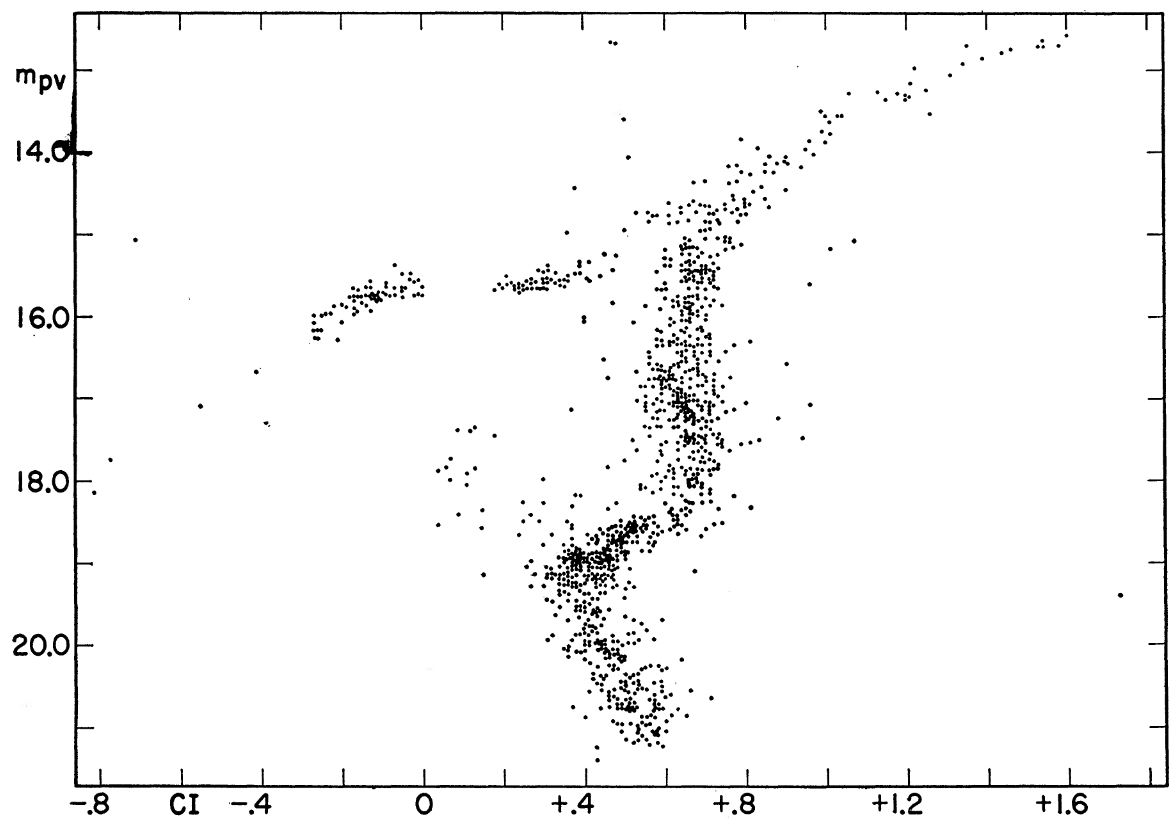
\includegraphics[width=0.75\textwidth]{src/Figures/Gould53.png}
	\caption{$m_{pg}$ - $m_{pv}$ color-magnitude diagram for the globular cluster M3.}
	\label{fig:M3CMD}
\end{figure}

Despite the canonical view of single populations composing GCs, there has been
spectroscopic evidence for chemical inhomogeneities in GCs since the early
1970s \citep[e.g.][]{Osborn1971} and by the late 1980s, as higher resolution
photometry became available, multiple clusters were known which exhibited
features in their CMDs consistent with either bimodal or multimodal stellar
populations \citep[e.g.][]{Norris1987}.

Conclusive evidence for MPs came from multiple observed red giant branches in
$\omega$Cen \citep{Lee1999}; however, this observation was not initially
believed to be generally characteristic of GCs \citep{Gnedin2002}. Just under a decade latter, with
Hubble Space Telescope (HST) high precision crowded field photometry in which
three distinct main sequences in NGC 2808 were identified \citep{Piotto2007},
the notion that GCs can have multiple populations became widespread. Since this
discovery, split main sequences have been found in nearly all Milky Way
globular clusters studied by HST \citep{anderson2009,milone2011}. Split stellar
populations are believed to be due to enhanced helium abundances, with
signifigant observed star-to-star light-element abundance variation, in their
stellar populations formed after the primordial population of stars
\citep{d2005,Piotto2007}. When compared to primordial helium mass fractions
($Y$) of $Y\sim 0.25$ \citep{collaboration2016planck} or solar helium
abundances $Y\sim0.27$ \citep{vinyoles2017new} these populations have mass
fractions as high as $Y\sim 0.4$. Helium enhancement is strongly suspected to
be the result of an earlier, more massive population dying off, enriching the
interstellar medium \citep{Gratton2001, Gratton2004, Gratton2012}; however,
precise formation channels for split stellar populations remain contentious. 

Two chapters of this thesis will further constrain the helium enhancement of
MPs within globular clusters by modeling their stellar populations in a fully
chemically self-consistent manner. Sections \ref{sec:p4} and
\ref{sec:p5} address the details of these projects in more detail.

\subsection{Local Solar Neighborhood}
\citet{Jao2018} discovered a novel feature in the Gaia $G_{BP}-G_{RP}$
color-magnitude-diagram. Around $M_{G}=10$ there is an approximately 17\%
decrease in stellar density of the sample of stars \citeauthor{Jao2018}
considered. Subsequently, this has become known as either the Jao Gap, or Gaia
M dwarf Gap. Section \ref{sec:p1} will go into more detail regarding the
physics underpinning this feature; however, in brief convective instabilities
in the core are believed to form for stars straddling the fully convective
transition mass (0.3 - 0.35 M$_{\odot}$) \citep{Baraffe2018}. These
instabilities result in stars' luminosities preferentially evolving either
slightly brighter or dimmer than the mass-luminosity relation around the
convective transition mass would naively indicate \citep{Jao2020}.

The Jao Gap, inherently a feature of M dwarf populations, provides an enticing
and unique view into the interior physics of these stars \citep{Feiden2021}.
This is especially important as, unlike more massive stars, M dwarf seismology
is currently infeasible due to the short periods and extremely small
magnitude's which both radial and low-order low-degree non-radial seismic waves
are predicted to have in such low mass stars \citep{Rodriguez-Lopez2019}. The
Jao Gap therefore provides one of the only current methods to probe the
interior physics of M dwarfs.

Stellar modeling has been successful in reproducing the Jao Gap
\citep[e.g.][]{Feiden2021,Mansfield2021} and, with these models, we have begun
to understand which parameters constrain the Jao Gap's location. For example,
it is now well documented that metallicity affects the Jao Gap's color, with
higher metallicity stellar populations showing the Jao Gap at consistently
higher masses / bluer colors \citep{Mansfield2021}.

Initial testing we have done using DSEP along with articles from both
\citeauthor{Feiden2021} and \citeauthor{Mansfield2021} demonstrates the Jao Gap's
location sensitivity to age, evolving to higher mass regions of the
mass-luminosity relation with population age. Per \citet{Mansfield2021} the
degree of this location evolution also does not seem to be strongly sensitive
to metallicity. Sections \ref{sec:p2} and \ref{sec:p3} of this proposal lay out
a plan to use this observed age dependence to age-date kinematically separated
populations in the solar neighborhood.
